\documentclass{beamer}

\usepackage{txfonts}
\usepackage{hyperref}

\hypersetup{colorlinks=false,linkbordercolor=red,linkcolor=green,pdfborderstyle={/S/U/W 1}}

\addtobeamertemplate{navigation symbols}{}{ \hspace{1em}    \usebeamerfont{footline}%
    \insertframenumber / \inserttotalframenumber }

\geometry{papersize={12.8cm,14cm}}
\usepackage{lipsum}

\makeatletter
\newenvironment<>{contdproof}[1][\proofname]{%
    \par
    \def\insertproofname{#1\@addpunct{.}}%
    \usebeamertemplate{proof begin}#2}
  {\usebeamertemplate{proof end}}
\makeatother


\setbeamertemplate{theorems}[numbered]

\newtheorem*{nonumdefinition}{Definition}
\newtheorem*{nonumproblem}{Problem}
\newtheorem*{nonumremark}{Remark}
\newtheorem{proposition}[theorem]{Proposition}


\usepackage{tikz}
\newcommand*\mycirc[1]{%
  \tikz[baseline=(C.base)]\node[draw,circle,inner sep=.7pt](C) {#1};\:
}


\newcommand\myheading[1]{%
  \par\bigskip
  {\color{blue}{\large #1}}\par\smallskip}

%\usetheme{Warsaw}
%\usetheme{Berkeley} %sample 1
\usetheme{Berlin} % sample 2
%\usetheme{AnnArbor} % sample 3

\let\otp\titlepage
\renewcommand{\titlepage}{\otp\addtocounter{framenumber}{-1}}



\title{Lecture 1 : The Mathematical Theory of Probability}
\author{}
\date{}


\begin{document}
\begin{frame}[plain]
\titlepage
\end{frame}
\begin{frame}
\frametitle{1. Introduction}

Today we will do \S2.1 and 2.2. We will skip Chapter 1.

We all have an intuitive notion of probability.

Let's see.

What is the probability of tossing two heads in a row with a fair coin?
\end{frame} 

\begin{frame}
\myheading{Method 1}

List {\it all} possible outcomes 
$$
\left\{\mycirc{$HH$}, \ HT, \ TH, \ TT\right\}
$$
so $P=?$.

\myheading{Question}

What did we just assume to arrive at that answer?
\end{frame}

\begin{frame}
\myheading{Another way}

\centerline{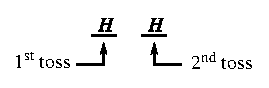
\includegraphics{figure/fig1.eps}}

However it is important to put probability into a formal mathematic framework for many reasons. 
\end{frame}

\begin{frame}
\myheading{1. Even ``elementary''}

Problems become too hard unless we can break them down into simpler problems using the rule of {\it Set Theory}.

\myheading{Examples}

Let's see how you can deal with these now and later.

(there is another reason which we will run into later - we often have infinite sets and need calculus e.g. financial math)
\end{frame}

\begin{frame}
\myheading{Problems}

\begin{enumerate}
\item What is the probability of getting {\it one} head in one hundred tosses of a fair coin?

\item What is the probability of getting 27 heads in one hundred tosses of a fair coin?
\end{enumerate}
Prediction - nobody will get this one now.

In two weeks everybody will.
\end{frame}

\begin{frame}
\myheading{2. Transition from the naive theory to the formal mathematical theory}

To make the transition we introduce the word ``experiment'' which will be taken to mean ``any action or process whose outcome is subject to uncertainty'' 

text - pg. 47.

\myheading{Examples}

Tossing a fair coin 100 times.

Dealing 5 cards from a 52 card deck - a poker hand.

Dealing 13 cards from a 52 card deck - a bridge hand.
\end{frame}

\begin{frame}
\begin{nonumdefinition}
The set of all possible outcomes of on experiment will be called the {\it sample space} of that experiment and denote $s$.
\end{nonumdefinition}

\myheading{Experiment}

3 tosses of a fair coin. 
$$
s=
\left\{
\begin{array}{c}
HHH, \ HHT, \ HTH, \ HTT,\\[4pt]
THH, \ THT, \ TTH, \ TTT
\end{array}
\right\}
$$
\end{frame}

\begin{frame}
\begin{nonumdefinition}
A subset $A$ of $s$ is called an event.
\end{nonumdefinition}


\begin{nonumproblem}
Find $P$ (at least one head in 3 tosses of a fair coin)
\end{nonumproblem}

We are looking for $P(A)$ where $A$ is a subset of the previous $s$.
\end{frame}

\begin{frame}
$$
s=\left\{HHH, \ HHT, \ HTH, \ HTT, \ THH, \ THT, \ TTH, \ TTT\right\}
$$

We will call this ``our favorite sample space'' from now on.
\end{frame}

\begin{frame}
\myheading{3. The Formal Mathematical Theory}

Let $s$ be a set (the sample space). A {\it probability measure} $P$ on $s$ is a rule (function) which assigns a real number $P(A)$ to any subset $A$ of $s$ (i.e., to any event) such that the following axioms are satisfied
\begin{enumerate}
\item For any event $A\subset s$ we have $P(A)\geq 0$

\item $P(s)=1$
\end{enumerate}
\end{frame}

\begin{frame}
\begin{enumerate}
\setcounter{enumi}{2}
\item If $A_{1}$, $A_{z}$,\quad, $A_{n}$,\ldots

is a possibly infinite collection of pairwise disjoint (mutually exclusive) events then 
$$
P\left(A,\cup A_{z}\cup\ldots\cup A_{n}\cup \ldots\right)=\underbrace{\sum\limits^{\infty}_{n=1}P(A_{n})}_{\substack{\text{sum of an infinite series}\\ \text{not just ordinary sum.}}}
$$
mutually exclusive means $A_{i}\cap A_{j}=\emptyset$ for any pair $i$, $j$ with $i\neq j$.
\end{enumerate}
\end{frame}

\begin{frame}
\myheading{Special cases}
\begin{enumerate}
\item Two mutually-exclusive events $A_{1}$ and $A_{2}$ (so $A_{1}\cap A_{2}=\emptyset$)
$$
P(A_{1}\cup A_{2})=P(A_{1})+P(A_{2})
$$

\item $n$ mutually-exclusive events $A_{1},A_{2},\ldots,A_{n}$
$$
P(A_{1}\cup A_{2}\cup\ldots\cup A_{n})=P(A_{1})+P(A_{2})+\cdots+P(A_{n})
$$
\end{enumerate}
\end{frame}

\begin{frame}
\myheading{A Class of Examples}

Let $s$ be a set with $n$ elements. Let $A\subset s$ be any subset. Define
$$
P(A)=\dfrac{\sharp (A)}{\sharp (s)}=\dfrac{\sharp(A)}{n}
$$
Then $P$ satisfies the axioms $1.$, $2.$ and $3$.

Here $\sharp (A)$ means the number elements in $A$. This is called the ``equally likely probability measure''.
\end{frame}

\begin{frame}
\myheading{An example in the above class}

Take our favorite sample space
$$
s=
\left\{
\begin{array}{c}
HHH, \ HHT, \ HTH, \ HTT\\[3pt]
THH, \ THT, \ TTH, \ TTT
\end{array}
\right\}
$$
Let $A$ be the subset (event) of outcomes with at least one head and one tail.

All the outcomes are equally likely (because the coin is fair) so
$$
P(A)=\dfrac{\sharp (A)}{\sharp (s)}=\dfrac{P}{8}
$$
\end{frame}

\begin{frame}
\myheading{A continuous Example 15}

Consider the unit square $s$ in the plane
\begin{center}
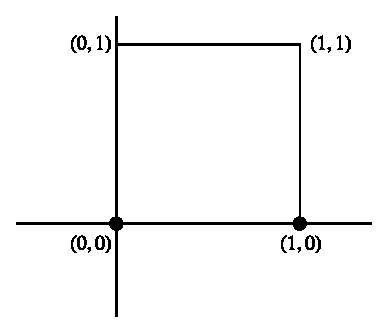
\includegraphics[scale=.8]{figure/fig2.eps}
\end{center}

Let $A\subset s$ be any subset.

Define
$$
P(A)=\text{Area of~ } A
$$
Then $P$ satisfies the axioms $1.$, $2.$ and $3$.
\end{frame}

\begin{frame}
Let $A$ be the subset of points in the square below the diagonal.

What is $P(A)$?

\centerline{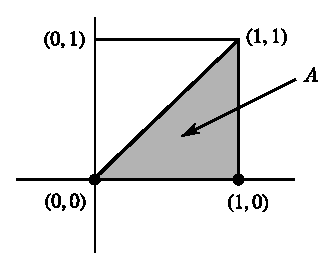
\includegraphics{figure/fig3.eps}}

Can you find $A$ so that $P(A)=\dfrac{1}{\pi}$?
\end{frame}

\begin{frame}
\myheading{4. A Quick Trip Through Set-Theory (pg. 49-50)}


Let $s$ be a set and $A$ and $B$ be subsets. Then we have $A\cup B$ (union), $A\cap B$ (intersection) and $A'$ (complement).

\myheading{Venn diagrams}

\centerline{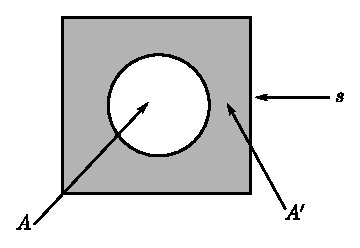
\includegraphics{figure/fig4.eps}}
\end{frame}

\begin{frame}
\centerline{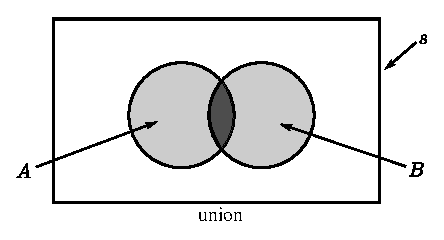
\includegraphics{figure/fig5.eps}}

\centerline{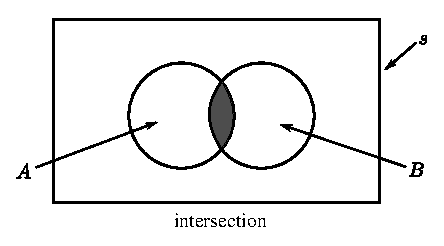
\includegraphics{figure/fig6.eps}}

\medskip

$A\cup B$ = ``everything in $s$ that is in either $A$ {\it or} $B$''

$A\cap B$ = ``everything in $s$ that is in $A$ {\it and} $B$''
\end{frame}

\begin{frame}
\myheading{The formulas linking $\cup$, $\cap$ and $'$}

To help you remember the formulas that follow use the analogy

$s \longleftrightarrow$ set of numbers

$\cup \longleftrightarrow +$

$\cap \longleftrightarrow \cdot$

\myheading{The commutative laws}

$A\cup B=B\cup A$ (analogue $a+b=b+a$)

$A\cap B=B\cap A$ (analogue $a\cdot b=b\cdot a$)
\end{frame}

\begin{frame}
\myheading{The associative laws}

$(A\cup B)\cup C=A\cup (B\cup C)$ (analogue $(a+b)+c=a+(b+c)$)

$(A\cap B)\cap C=A\cap(B\cap C)$ (analogue $(a\cdot b)\cdot c=a-(b\cdot c)$)

Now we have laws that relate two or more of $\cup$, $\cap$ and $'$.

\myheading{The distributive laws}

$A\cap (B\cup C)=(A\cap B)\cup (A\cap C)$ (analogue $a-(b+c)=(a\cdot b)+(a\cdot c)$)

$A\cap (B\cap C)=(A\cup B)\cap (A\cup C)$ no analogue

\begin{nonumproblem}
What would the analogue of the second distributive law say. It isn't true.
\end{nonumproblem}
\end{frame}

\begin{frame}
\myheading{De Morgan's Laws}

(no analogy with $+$, $\cdot$)

$(A\cup B)'=A'\cap B'$

$(A\cap B)'=A'\cup B'$

\begin{tabular}{@{}c}
$C\subset D\Leftrightarrow C'\supset D'$\\
$\uparrow$\\
if and only if
\end{tabular}

(so complement reverses $\cup$, $\cap$ and $\subset$)

One way to think of the first formula

not in $A$ or $B$ = not in $A$ and not in $B$
\end{frame}

\begin{frame}

The best way to see it is by a Venn diagram

\smallskip

\includegraphics{figure/fig7.eps}

\smallskip

\qquad~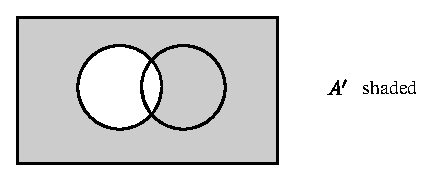
\includegraphics{figure/fig8.eps}

\smallskip

\qquad~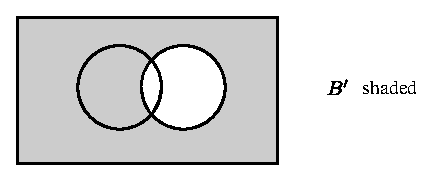
\includegraphics{figure/fig9.eps}

\smallskip

Top square = intersection of bottom two squares
\end{frame}

\begin{frame}

\myheading{Consequences of the axioms of probability theory}

pg. 54-56.

We will prove two propositions which will be {\em extremely useful} to you.

\begin{proposition}[Complement law]\label{art1-prop1}
$$
P(A')=1-P(A).
$$
\end{proposition}

\begin{contdproof}
$A\cup A'=s$ so

$P(A\cup A')=P(s)=1$ (axiom 2) ($\sharp$)

But $A\cap A'=\emptyset$ so by
\end{contdproof}
\end{frame}

\begin{frame}
\begin{proof}[Proof (Cont.)]
axiom 3, special case 1
$$
P(A\cup A')=P(A)+P(A')\quad (\sharp\sharp)
$$
Putting $(\sharp)$ and $(\sharp\sharp)$ together we get
$$
1=P(A)+P(A')
$$
\end{proof}

\setcounter{theorem}{0}
\begin{corollary}
$P(\phi)=0$.
\end{corollary}

\begin{proof}
$\phi=s'$

so $P(\phi)=1-P(s)=1-1=0$.
\end{proof}
\end{frame}

\begin{frame}
\begin{nonumremark}
$\emptyset$ is not the Greek letter phi, it is a Norwegian letter. The symbol was chosen by Andr\'e Weil.
\end{nonumremark}

\begin{corollary}
$P(A)\leq 1$.
\end{corollary}

\begin{proof}
$P(A)=1-P(A')\leq 1$

because $P(A')\geq 0$.
\end{proof}

\myheading{Bottom line (literally)}
$$
0\leq P(A)\leq 1
$$

\end{frame}

\begin{frame}
To illustrate the use of Proposition \ref{art1-prop1}, let us go back to computing $P$ (at least one head in three tosses)

Put $s$ = our favorite sample space.

$A$ = at least one head {\bf SO}

$A'$ = no heads = all tails = $TTT$

so
$$
P(A)=1-P(TTT)=1-\dfrac{1}{8}=\dfrac{7}{8}
$$
Now we can do 100 tosses

$P$ (at least one head) $=1-\dfrac{1}{100}=\dfrac{99}{100}$
\end{frame}

\begin{frame}
Recall that two events $A$ and $B$ are mutually exclusive if $A\cap B=\emptyset$ and axiom 3 says in this case
$$
P(A\cup B)=P(A)+P(B) \ (\sharp)
$$
The following proposition is absolutely critical for computations

\setcounter{theorem}{1}
\begin{proposition}[Additive Law]\label{art1-prop2}
$P(A\cup B)=P(A)+P(B)-P(A\cap B)$
\end{proposition}
Note that this is consistent with $(\sharp)$ above because if $A\cap B=\emptyset$ then
$$
P(A\cap B)=P(\emptyset)=0
$$
\end{frame}

\begin{frame}
\begin{contdproof}
The proof is hard.

It depends on the following Venn diagram.

\smallskip
\centerline{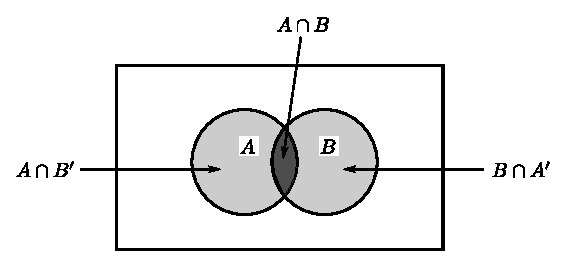
\includegraphics{figure/fig10.eps}}
\smallskip

We see that $A\cup B$ is the union of three {\it mutually exclusive} sets.
$$
A\cup B=(A\cap B')\cup (A\cap B)\cup (B\cap A')
$$
so by axiom 3 with $n=3$
$$
P(A\cup B)=P(A\cap B')+P(A\cap B)+P(B\cap A') \ (\sharp\sharp)
$$
\end{contdproof}
\end{frame}

\begin{frame}
\begin{proof}[Proof (Cont.)]
How do we compute the first and third terms?

We have a disjoint union (i.e., union of mutually exclusive sets)
$$
A=(A\cap B)\cup (A\cap B')
$$

\centerline{\includegraphics[scale=.85]{figure/fig11.eps}}

so by axiom 3
$$
P(A)=P(A\cap B)+P(A\cap B')
$$
whence
\begin{equation*}
P(A\cap B')=P(A)-P(A\cap B)\tag{1}\label{art1-eq1}
\end{equation*}
Similarly
\begin{equation*}
P(B\cap A')=P(B)-P(A\cap B)\tag{3}\label{art1-eq3}
\end{equation*}
Plug \eqref{art1-eq1} and \eqref{art1-eq3} into $(\sharp\sharp)$.
\end{proof}
\end{frame}

\begin{frame}
What about the intersection of three terms?

\begin{proposition}\label{art1-prop3}
\begin{gather*}
P(A\cup B\cup C)=P(A)+P(B)+P(C)\\
-P(A\cap B)-P(A\cap C)-P(B\cap C)\\
+P(A\cap B\cap C)
\end{gather*}
This is (more or less) ``the principle of exclusion and inclusion''
\begin{enumerate}
\item {\it include} the singletons $A$, $B$, $C$

\item {\it exclude} the pairs $A\cap B$, $A\cap C$, $B\cap C$

\item {\it include} the triple $A\cap B\cap C$
\end{enumerate}
\end{proposition}
\end{frame}

\end{document}


